\subsection{Gate dell'ADC}

Variamo la durata del gate dell'ADC e calcoliamo il rapporto $\sigma\!/$\!media per il picco di annichilazione rivelato dal PMT1, modellato come al solito con una gaussiana.
Su alcune misure abbiamo introdotto dei ritardi per migliorare o peggiorare la sincronizzazione con il gate al fine di quantificare quanto la messa in tempo influisca sulla nostra risoluzione. Il risultato di questa misura è in \autoref{fig:gate}, i dati sono in \autoref{tab:gate}.

\begin{figure}[h]
\centering
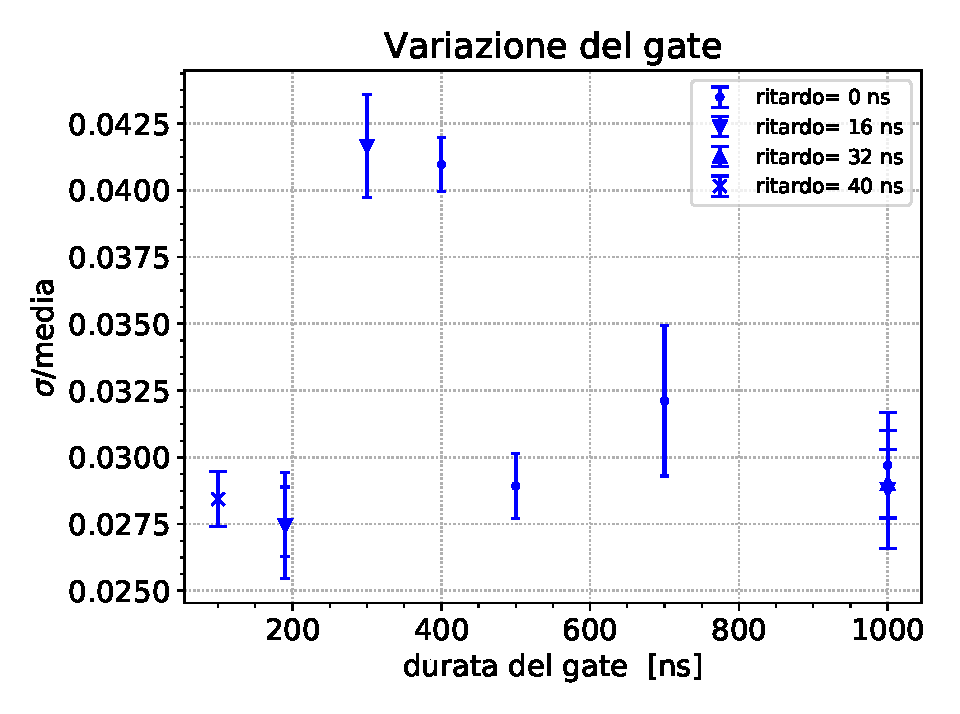
\includegraphics[width=20 em]{immagini/gate}
\caption{Grafico della risoluzione in funzione della durata del gate. Le misure sovrapposte sono state ottenute ritardando il segnale del PMT1.}
\label{fig:gate}
\end{figure}

\begin{table}[h]
\centering
\begin{tabular}{c|c|c|c}
durata (ritardo) [ns] & media [digit] & $\sigma$ [digit] & $\sigma\!/$\!media\\
\hline
 100 (40) & 304.88\,$\pm$\,0.34 & 307.68\,$\pm$\,0.36 &  1.0092\,$\pm$\,0.0016 \\
 190 (16) & 492.82\,$\pm$\,0.50 & 344.25\,$\pm$\,0.25 & 0.69853\,$\pm$\,0.0008 \\
 190 & 513.05\,$\pm$\,0.80 & 524.01\,$\pm$\,0.42 &  1.0213\,$\pm$\,0.0018 \\
 300 & 307.68\,$\pm$\,0.36 & 482.54\,$\pm$\,0.85 &  1.5683\,$\pm$\,0.0033 \\
 400 & 344.25\,$\pm$\,0.25 & 539.43\,$\pm$\,0.61 &  1.5670\,$\pm$\,0.0021 \\
 500 & 524.01\,$\pm$\,0.42 & 553.88\,$\pm$\,0.71 &  1.0570\,$\pm$\,0.0016 \\
 700 & 482.54\,$\pm$\,0.85 & 542.68\,$\pm$\,0.41 &  1.1247\,$\pm$\,0.0022 \\
1000 (16) & 539.43\,$\pm$\,0.61 & 304.88\,$\pm$\,0.34 & 0.56519\,$\pm$\,0.0009 \\
1000 (0) & 553.88\,$\pm$\,0.71 & 492.82\,$\pm$\,0.50 &  0.8898\,$\pm$\,0.0014 \\
1000 (32) & 542.68\,$\pm$\,0.41 & 513.05\,$\pm$\,0.80 &  0.9454\,$\pm$\,0.0016 
\end{tabular}

\caption{Andamento della risoluzione in funzione della durata del gate. I numeri tra parentesi indicano di quanto è stato ritardato il PMT1.}
\label{tab:gate}
\end{table}

Dall'analisi dei dati abbiamo potuto vedere che la risoluzione migliore si raggiunge quando il gate dura meno di \SI{200}{ns}, ma questo valore non è un buon punto di lavoro perché cambiare la durata del gate cambia la scala e, in questo caso, non ci permetteva di vedere il picco del neon. L'alternativa migliore sembrerebbe essere una durata del gate di \SI{1}{\micro s}, ma il manuale dell'ADC specifica che a tale valore (o anche maggiore) diminuisce la linearità della digitalizzazione. Per questo abbiamo scelto di usare un gate di \SI{550}{ns} nell'apparato A. Questa scelta è poi diventata \SI{1}{\micro s} nell'apparato B per evitare problemi derivanti dal jitter dei segnali. Infine notiamo che cambiare i ritardi sui segnali in ingresso non influisce significativamente sulla risoluzione dell'apparato.